\documentclass[12pt, a4paper, oneside]{book}
\usepackage[hidelinks]{hyperref}
\usepackage[british,UKenglish,USenglish,english,american]{babel}
\usepackage{epsfig}
\usepackage{epstopdf}
\usepackage[chapter]{algorithm}
\usepackage{algorithmic}
\usepackage{listings}
\usepackage{amsmath}
\usepackage{amssymb}
\usepackage{graphicx}
\usepackage{multirow}
\usepackage{color}
\usepackage{url}
\usepackage{siunitx}
\usepackage[utf8]{inputenc}
\usepackage[T1]{fontenc}
\usepackage{setspace}
\usepackage{tabularx}
\usepackage{textcomp}
\usepackage{caption}
\usepackage{natbib}
\usepackage{textcomp}
\usepackage{multirow}

\setstretch{1.5}
%\renewcommand\baselinestretch{1.5} % riadkovanie jeden a pol

% pekne pokope definujeme potrebne udaje
\newcommand{\mftitle}{Development of an efficient tracklet building algorithm for space debris objects}
\newcommand{\mfthesistype}{Diplomová práca}
\newcommand{\mfauthor}{Bc. Stanislav Krajčovič}
\newcommand{\mfadvisor}{prof. RNDr. Roman Ďurikovič, PhD.}
\newcommand{\mfplacedate}{Bratislava, 2018}
\newcommand{\mfuniversity}{UNIVERZITA KOMENSKÉHO V BRATISLAVE}
\newcommand{\mffaculty}{FAKULTA MATEMATIKY, FYZIKY A INFORMATIKY}
\newcommand{\sub}[1]{$_{\text{#1}}$}
\newcommand{\reference}[1]{č.~\ref{#1}}
\newcommand{\imageHeight}{150px}
%\newcommand{\tit1}{Development of an efficient tracklet }
%\newcommand{\tit2}{building algorithm for space debris objects}

\DeclareMathOperator{\arctantwo}{arctan2}
\captionsetup[table]{position=bottom}

\ifx\pdfoutput\undefined\relax\else\pdfinfo{ /Title (\mftitle) /Author (\mfauthor) /Creator (PDFLaTeX) } \fi

\begin{document}

\frontmatter

\thispagestyle{empty}

\noindent
\begin{minipage}{\textwidth}
\begin{center}
\textbf{\mfuniversity \\
\mffaculty}
\end{center}
\end{minipage}

\vfill
\begin{figure}[!hbt]
	\begin{center}
		
\includegraphics{images/logo_fmph}
		\label{img:logo}
	\end{center}
\end{figure}
\begin{center}
	\begin{minipage}{0.8\textwidth}
		\centerline{\textbf{\Large\MakeUppercase{Development of an efficient tracklet building }}}
		\smallskip
		\centerline{\textbf{\Large\MakeUppercase{algorithm for space debris objects}}}
		\bigskip
		\centerline{\textbf{\Large\MakeUppercase{Vývoj algoritmu na efektívne konštruovanie }}}
		\smallskip
		\centerline{\textbf{\Large\MakeUppercase{trackletov vesmírneho odpadu}}}
		\bigskip
		\bigskip
		\centerline{\mfthesistype}
	\end{minipage}
\end{center}
\vfill
2018 \hfill
\mfauthor
\eject 
% koniec obalu

\thispagestyle{empty}

\noindent
\begin{minipage}{\textwidth}
\begin{center}
\textbf{\mfuniversity \\
\mffaculty}
\end{center}
\end{minipage}

\vfill
\begin{figure}[!hbt]
\begin{center}

\includegraphics{images/logo_fmph}
\label{img:logo}
\end{center}
\end{figure}
\begin{center}
\begin{minipage}{0.8\textwidth}
		\centerline{\textbf{\Large\MakeUppercase{Development of an efficient tracklet building }}}
		\smallskip
		\centerline{\textbf{\Large\MakeUppercase{algorithm for space debris objects}}}
		\bigskip
		\centerline{\textbf{\Large\MakeUppercase{Vývoj algoritmu na efektívne konštruovanie }}}
		\smallskip
		\centerline{\textbf{\Large\MakeUppercase{trackletov vesmírneho odpadu}}}
		\bigskip
		\bigskip
		\centerline{\mfthesistype}
\end{minipage}
\end{center}
\vfill
\begin{tabular}{l l}
Study programme: & Applied Informatics\\
Field of study: & 2511 Applied Informatics\\
Department: & Department of Applied Informatics\\
Supervisor: & \mfadvisor \\
Consultant: & Mgr. Jiří Šilha, PhD.
\end{tabular}
\vfill
\noindent
\mfplacedate \hfill
\mfauthor
\eject 
% koniec titulneho listu

\thispagestyle{empty}

\begin{figure}[H]
\begin{center}
\makebox[\textwidth]{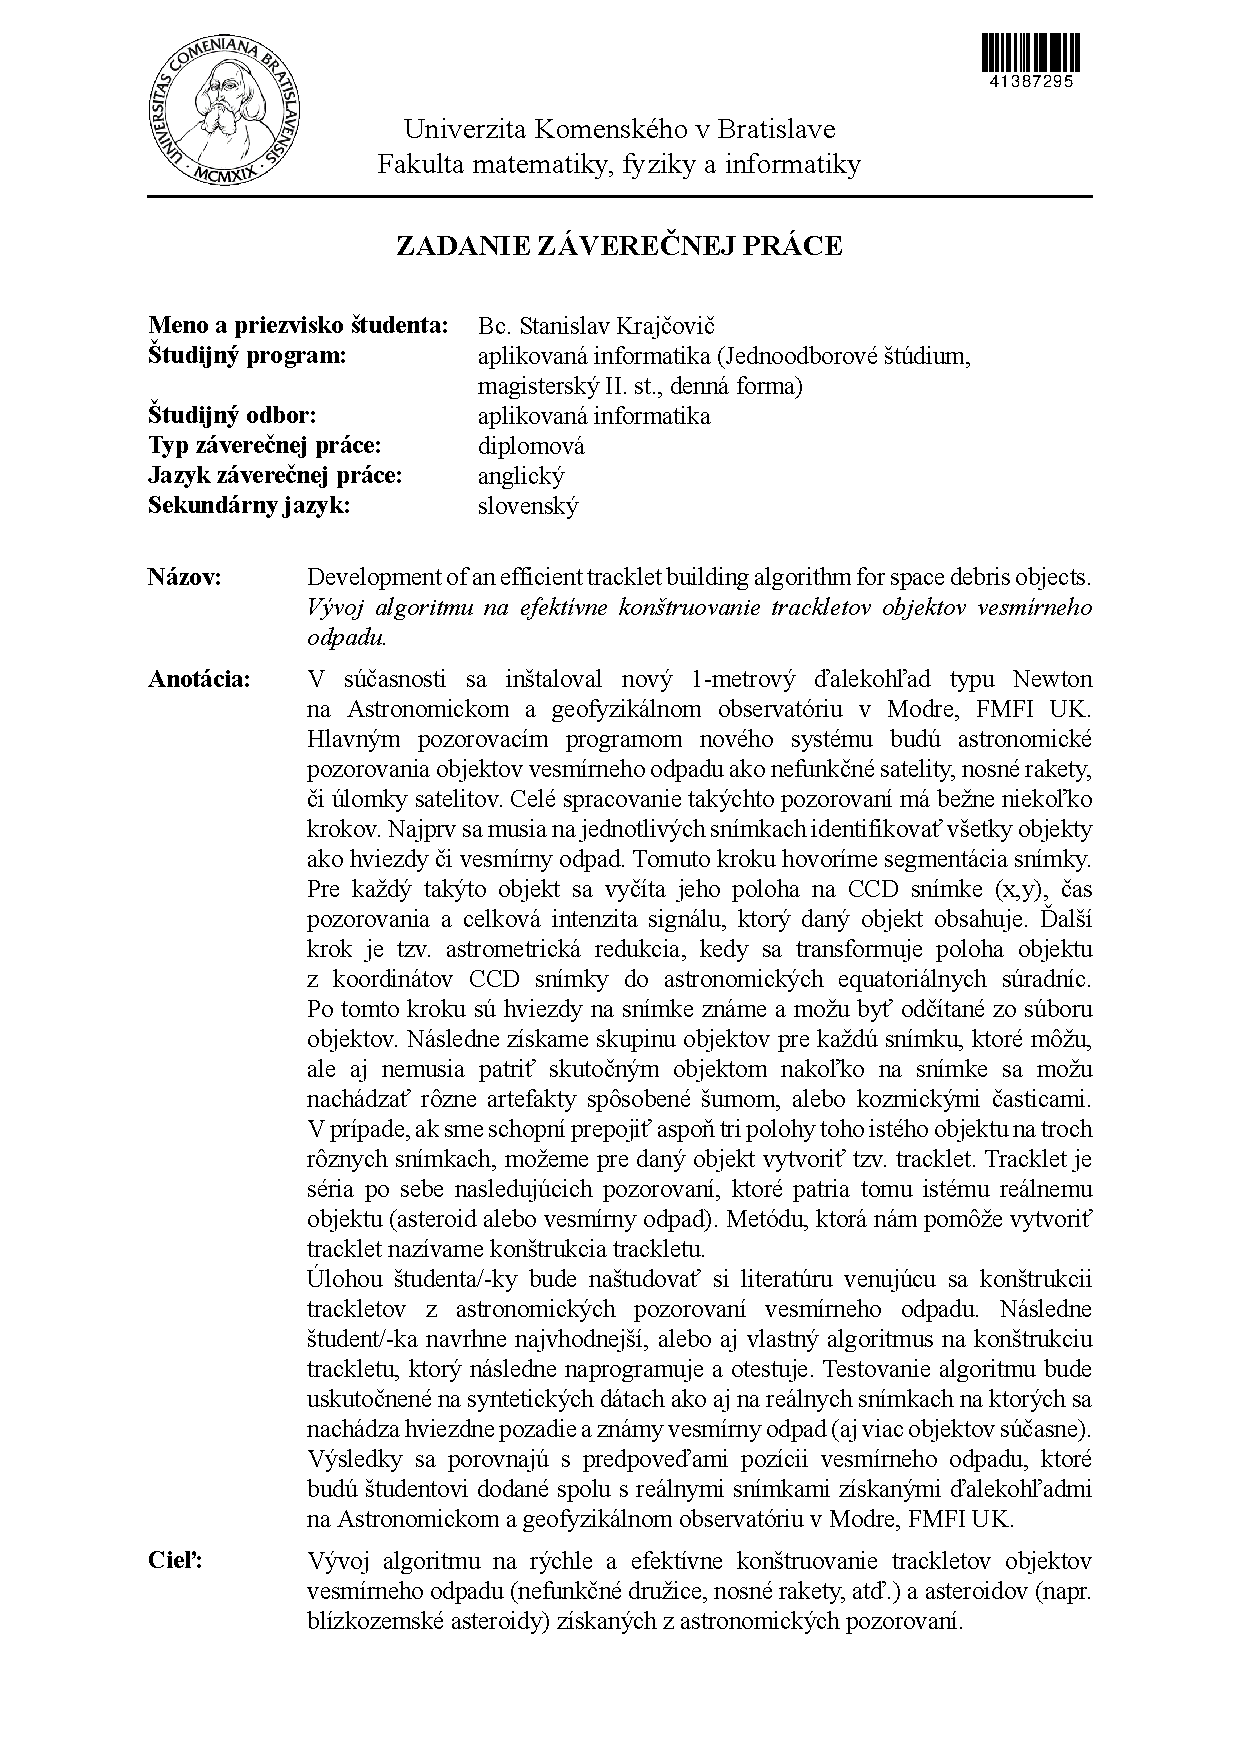
\includegraphics[page=1,width=18cm]{images/zadanie.pdf}}
\label{img:zadanie}
\end{center}
\end{figure}

\newpage

\thispagestyle{empty}

\begin{figure}[H]
\begin{center}
\makebox[\textwidth]{\includegraphics[page=2,width=18cm]{images/zadanie.pdf}}
\label{img:zadanie}
\end{center}
\end{figure}

{~}\vspace{12cm}

\noindent
\begin{minipage}{0.25\textwidth}~\end{minipage}
\begin{minipage}{0.75\textwidth}
I hereby certify that this thesis has been composed by me and is based on my work, unless stated otherwise. No other person's work has been used without due acknowledgement in this thesis. All references and verbatim extracts have been quoted, and all sources of information, including graphs and data sets, have been specifically acknowledged.
\newline \newline
\end{minipage}
\vfill
~ \hfill {\hbox to 6cm{\dotfill}} \\
\mfplacedate \hfill \mfauthor
\vfill\eject 

\chapter*{Acknowledgement}\label{chap:thank_you}
I would like to thank my supervisor, prof. RNDr. Roman Ďurikovič, PhD. for all his invaluable and expert advice and guidance, which helped me successfully finish this thesis. I would also like to thank my consultant, Mgr. Jiří Šilha, PhD. for provided knowledge about astronomy and astrodynamics; for all his advice and support. I must also thank my colleagues from the YACGS seminary for their patience and input.
\vfill\eject 

\chapter*{Abstract}\label{chap:abstract_en}
Astronomical observations of a specific portion of the night sky produce images saved in Flexible Image Transport System (FITS) format. They contain basic information such as date, exposure time and other. However, these files are processed in a complex pipeline beforehand and data about the objects inside is gained. This document contains summary of prerequisite knowledge needed, such as the theory behind object dynamics, already existing solutions and an analysis of inputs. Then, we describe the design and creation of algorithms used to create tracklets, which are observations of the same object in time. We describe our reasoning behind using linear regression, Initial Orbit Determination and not using Hough transform. The implementation, including methods and class variables, follows. In conclusion, we review the effectiveness of our implementation and suggest possible improvements.

~\\
Keywords: space debris, observation, tracklet
\vfill\eject 

\chapter*{Abstrakt}\label{chap:abstract_sk}
Astronomickými pozorovaniami časťami nočnej oblohy získavame obrázky uložené v tzv. Flexible Image Transport System (FITS) formáte. Obsahujú základné dáta, ako dátum, čas expozície a iné. Tieto súbory sú avšak spracované v komplexnom systéme a tým sú získané informácie o objektoch na snímkach. Tento dokument obsahuje zhrnutie potrebných vedomostí, ako napríklad dynamiku telies, existujúcich riešení a analýzu vstupných dát. V ďalšom kroku popisujeme dizajn a tvorbu algoritmov použitých na tvorbu trackletov, čo sú vlastne pozorvania toho istého objektu v čase. Zároveň odôvodňujeme dôvody na použitie lineárnej regresie, algoritmu Initial Orbit Determination a dôvod na vynechanie algoritmu Hough transform. Po tejto časti nasleduje implementácia, ktorá zahŕňa metódy a triedne premenné. Na záver zhrnieme efektivitu našej implementácie a navrhneme možné vylepšenia.

~\\
Kľúčové slová: vesmírny odpad, pozorovanie, tracklet
\vfill\eject 
% koniec abstraktov

\tableofcontents

\mainmatter

% treba este prejst dokument ci je kod spravne formatovany
\input 01uvod.tex
\input 02introduction.tex
\input 03object_dynamics.tex
\input 04existing_solutions.tex
\input 05requirements.tex
\input 06proposed_solutions.tex
\input 07design_implementation.tex
\input 08results.tex
\input 09conclusion.tex

\backmatter

\nocite{*}
\bibliographystyle{apalike}
\bibliography{references}

\end{document}